%*******************************************************************************
% Macro per il documento corrente
%*******************************************************************************
\newcommand{\sharedPath}{../shared}
\newcommand{\doctitle}{Piano di Progetto}


%*******************************************************************************
% Preambolo
%*******************************************************************************
\documentclass[a4paper,10pt,twoside]{book}

%*******************************************************************************
% Codifica e lingua
%*******************************************************************************
\usepackage[utf8x]{inputenc}
\usepackage[T1]{fontenc}
\usepackage[english,italian]{babel}
\usepackage{lmodern}
\usepackage{multirow}
\usepackage{amsmath,eurosym}
%*******************************************************************************
% Qualche macro utile a tutti
%*******************************************************************************
\newcommand{\docRoot}{..}
\newcommand{\inglese}[1]{\foreignlanguage{english}{\textit{#1}}}
\newcommand{\team}{\textsf{EtaBeta\,Software}\xspace}
\newcommand{\caName}{BPM-1.0\xspace}
\newcommand{\customer}{\textsf{Alpha\,\&\,Partners}\xspace}
\newcommand{\mktg}{\inglese{marketing}\xspace}
\newcommand{\bsn}{\inglese{business}\xspace}
\newcommand{\sw}{\inglese{software}\xspace}

%*******************************************************************************
% Figure e immagini
%*******************************************************************************
\usepackage{graphicx}
\graphicspath{{\docRoot/shared/pictures/}}

%*******************************************************************************
% Tabelle
%*******************************************************************************
\usepackage{booktabs}
\usepackage{array}

%*******************************************************************************
% Elenchi puntati personalizzati
%*******************************************************************************
\usepackage{enumitem}

%*******************************************************************************
% Landscape per ruotare le pagine
%*******************************************************************************
\usepackage{pdflscape}

%*************************************************
% Collegamenti intra- e intertestuali
%*************************************************
\usepackage{hyperref}
\hypersetup{%
    colorlinks=false,linktocpage=false,pdfborder={0 0 0},%
    pdfstartpage=1, pdfstartview=FitV,plainpages=false,%
    urlcolor=Black, linkcolor=Black,
    pdfcreator={pdfLaTeX},%
    pdfproducer={pdfLaTeX with hyperref package}%
}

%*************************************************
% Grafica vettoriale
%*************************************************
\usepackage{tikz}
\usetikzlibrary{shadows,arrows,shapes}

%*******************************************************************************
% Altri pacchetti
%*******************************************************************************
\usepackage{xspace} % per spazi condizionali extra
\usepackage{lastpage} % per sapere il numero totale di pagine
\usepackage{microtype} % qualche accorgimento tipografico

% *************************************************
% Intestazioni e piè di pagina personalizzati
% *************************************************
\usepackage{fancyhdr}

% stile normale
\fancypagestyle{normal}{
\fancyhead{}
\fancyhead[RE,LO]{
\sffamily\team
}
\fancyhead[LE,RO]{
\sffamily\leftmark
}
\renewcommand{\headrulewidth}{.4pt}
\cfoot{}
\fancyfoot[LE,RO]{\sffamily
  pag. \thepage{} di \pageref{LastPage}}
\fancyfoot[RE,LO]{\sffamily\doctitle}
\renewcommand{\footrulewidth}{.4pt}
}

% stile per gli indici
\fancypagestyle{toc}{
\fancyhead{}
\renewcommand{\headrulewidth}{0pt}
\cfoot{}
\fancyfoot[RO,LE]{\sffamily\thepage{}}
\fancyfoot[RE,LO]{\sffamily\doctitle{}}
\renewcommand{\footrulewidth}{.4pt}
}

\pagestyle{fancy}
\renewcommand{\sectionmark}[1]{\markboth{#1}{#1}}


%*******************************************************************************
% Inizio documento
%*******************************************************************************
\begin{document}

\pagestyle{empty}
\begin{center}

{\sffamily
Sviluppo e Gestione Progetti\\
a.a. 2012--2013
}

\vskip 1.5cm

{
\setlength{\fboxsep}{.2pt}
\fbox{
\includegraphics[width=\textwidth]{logo}}
}

\vskip .5cm

{\Huge\sffamily\bfseries
\team
}

\vskip 1.5cm

% titolo del progetto
{\Large\sffamily\bfseries
\caName
}

\vskip 1cm

% titolo del documento
\hrule
\vskip 10pt
{\Huge\scshape
\doctitle
}
\vskip 10pt
\hrule

\end{center}

\clearpage
\pagenumbering{roman} 

\tableofcontents{\thispagestyle{toc}}

\clearpage

\pagestyle{normal}
\pagenumbering{arabic}




\section{Introduzione}


\subsection{Scopo del documento}


\section{Pianificazione}
\subsection{Work Breakdown Structure}

La Work Breakdown Structure (WBS) costituisce il primo passo verso una buona pianificazione.

La WBS sfrutta il concetto di \textit{``Divide ed Impera''}; essa infatti ha lo scopo di suddividere il lavoro di progetto in parti minori: in questo modo anche i progetti più complessi diventano realizzabili.

La scomposizione avviene in modo gerarchico: il lavoro viene suddiviso in attività che a loro volta vengono scomposte in sotto attività più piccole e semplici da gestire, dette Work Package (WP).
La rappresentazione della scomposizione avviene tramite l'uso di un albero, dove i nodi sono le attività e le foglie i WP.

La WBS permette, tramite la suddivisione del lavoro in segmenti minori, di analizzare tutte le implicazioni del progetto senza tralasciare nulla. Inoltre, costituisce anche un buon punto di partenza per calcolare costi e benefici del progetto.
La WBS offre una chiara visione del prodotto finale e del processo complessivo attraverso il quale è stato creato il prodotto.


Si presenta di seguito la definizione della WBS per il progetto ....%TODO questo va scritto alla fine, non si può fuffare ora!
Ogni sezione riporta la descrizione dell'attività di primo livello e la descrizione relativa ad ogni suo WP. 

		Il team ha scelto di strutturare la WBS seguendo il ciclo di vita del progetto.
		\begin{figure}[!h]
  		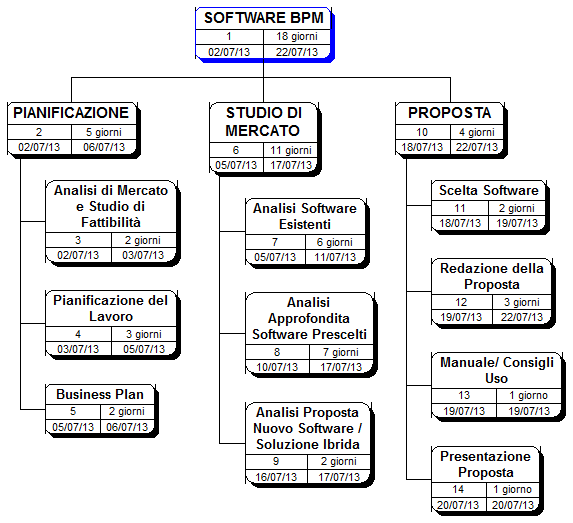
\includegraphics[width=\textwidth]{WBS}
		\caption{Work Breakdown Structure}
		\end{figure}

\clearpage


		\subsubsection{Pianificazione}
		In questa fase devono essere eseguite tutte le attività necessarie alla pianificazione del progetto.
		Devono essere individuate ed organizzate tutte le attività da svolgere, i tempi e le risorse necessarie allo sviluppo del progetto. Tale fase comprende anche la stesura del \inglese{Business Plan}.
		
		\paragraph{Analisi di Mercato e Studio di Fattibilità}

		\begin{itemize}
		\item{\bfseries Descrizione:} 
		questo WP prevede uno studio generale del mercato sui \inglese{software} BPM, con lo scopo di permettere l'organizzazione della pianificazione in base alle informazioni tratte dagli studi.
In particolare, lo studio di fattibilità dà al \inglese{team} la possibilità di capire se gli strumenti e le risorse di cui dispone sono sufficienti a garantire il conseguimento dell'obbiettivo.
L'analisi, invece, permette di eseguire una corretta pianificazione sulla base di informazioni reali riguardanti il mercato attuale. 
		\item {\bfseries Responsabile:}
		\item  {\bfseries Attività:}
			\begin{itemize}
				\item Ricerche in rete
				\item Analisi ad alto livello delle funzionalità dei \inglese{software} BPM
				\item Ricerche brevettuali
			\end{itemize}
		\item  {\bfseries Costo:}
		\item  {\bfseries Tempo di realizzazione: }2 giorni lavorativi
		\end{itemize}



\paragraph{Pianificazione del Lavoro}
\begin{itemize}
\item{\bfseries Descrizione:} Questa attività prevede la pianificazione del lavoro in seguito allo studio di fattibilità effettuato. Il lavoro deve essere organizzato nelle sue attività e nei suoi tempi.
\item {\bfseries Responsabile:}
\item  {\bfseries Attività:}
	\begin{itemize}
		\item Stesura WBS
		\item Stesrua OBS
		\item Matrice delle responsabilità
		\item Stesrua RBS
		\item Diagramma di Gantt	
	\end{itemize}

\item  {\bfseries Costo:}
\item  {\bfseries Tempo di realizzazione:} 2 giorni lavorativi
\end{itemize}


\paragraph{Redazione Business Plan}
\begin{itemize}
\item{\bfseries Descrizione:} Questo WP prevede la redazione del Business Plan. Tale documento è molto importante sia a titolo organizzativo che rappresentativo, del progetto e dell'azienda stessa.
\item {\bfseries Responsabile:}
\item  {\bfseries Attività:}
\item  {\bfseries Costo:}
\item  {\bfseries Tempo di realizzazione:} 2 giorni lavorativi
\end{itemize}


\subsubsection{Studio di Mercato}
In questa fase devono essere eseguite tutte le attività inerenti allo studio di mercato sui \inglese{software} BPM.
Il primo passo da compiere è l'analisi generica del mercato e l'individuazione dei prodotti esistenti. Sarà poi necessario selezionare alcuni \inglese{software} atti all'analisi approfondita in modo tale da poter scegliere la migliore soluzione. 

\paragraph{Studio dei Software Esistenti }
\begin{itemize}
\item{\bfseries Descrizione:} Questo WP prevede l'analisi dei \inglese{software} già presenti nel mercato. Si tratta di analizzare le diverse soluzioni già esistenti in commercio ed individuare quelle più adatte all'obbiettivo del progetto. 

\item {\bfseries Responsabile:}
\item  {\bfseries Attività:}
		\begin{itemize}
		\item Analisi generica delle soluzioni \inglese{software} già presenti nel mercato
		\item Selezione di una lista di \inglese{software} da visionare
		\item Analisi generale dei \inglese{software}
		\end{itemize}

\item  {\bfseries Costo:}
\item  {\bfseries Tempo di realizzazione:} 6 giorni lavorativi
\end{itemize}

\paragraph{Studio dei Software Prescelti}
\begin{itemize}
\item{\bfseries Descrizione:}  Questo WP prevede l'analisi dei \inglese{software} selezionati. Si tratta di analizzare, studiare e confrontare le prestazioni dei vari software. Le caratteristiche che si terranno in considerazione sono:

%TODO
\item {\bfseries Responsabile:}
\item  {\bfseries Attività:}
\begin{itemize}

		\item Individuazione della lista degli aspetti da tenere in considerazione
		\item Analisi individuale di ogni \inglese{software}
		\item Confronto dei diversi \inglese{software}
		\end{itemize}

\item  {\bfseries Costo:}
\item  {\bfseries Tempo di realizzazione:} 7 giorni lavorativi
\end{itemize}


\paragraph{Analisi Proposta Nuovo Software o Soluzione Ibrida }
\begin{itemize}
\item{\bfseries Descrizione:} Qusto WP prevede l'analisi della possibilità della realizzazione di un nuovo \inglese{software} o di una soluzione ibrida. Tale analisi avverrà soltanto dopo aver esaminato i diversi \inglese{software} selezionati e la scelta sarà scaturita dalla possibilità che nessun \inglese{software} attualmente in commercio soddisfi pienamente le richieste.
\item {\bfseries Responsabile:}
\item  {\bfseries Attività:}
\item  {\bfseries Costo:}
\item  {\bfseries Tempo di realizzazione:} 2 giorni lavorativi
\end{itemize}




\subsubsection{Proposta}
In questa fase devono essere eseguite tutte le attività inerenti alla stesura delle proposta. Deve essere scelto il prodotto da proporre e individuato il modo per farlo. Si prevede inoltre di realizzare un piccolo manuale per l'uso del prodotto \inglese{software}.

\paragraph{Scelta Software }
\begin{itemize}
\item{\bfseries Descrizione:} Questo WP rappresenta un punto cruciale. Dalla scelta del \inglese{software} dipende il contenuto della proposta che sarà presentata. Si tratta quindi di decidere  nel migliore dei modi quel'è il \inglese{software} BPM più adatto alle esigenze richieste.
\item {\bfseries Responsabile:}
\item  {\bfseries Attività:}
\item  {\bfseries Costo:}
\item  {\bfseries Tempo di realizzazione:} 2 giorni lavorativi
\end{itemize}

\paragraph{Redazione della Proposta }
\begin{itemize}
\item{\bfseries Descrizione:} Una volta che la scelta del \inglese{software} è avvenuta, sarà necessario presentarla in modo formale all'azienda richiedente. Si noti che la forma con cui presentiamo il lavoro svolto è fondamentale per avere successo e portare a termine gli obiettivi prefissati.
\item {\bfseries Responsabile:}
\item  {\bfseries Attività:}
	\begin{itemize}
	\item Individuazione del contenuto della proposta
	\item Stesura del documento
	\item Verifica del documento
 	\item Approvazione del documento	
	\end{itemize}

\item  {\bfseries Costo:}
\item  {\bfseries Tempo di realizzazione:} 2 giorni lavorativi
\end{itemize}



\paragraph{Redazione Manuale/Consigli d'uso}
\begin{itemize}
\item{\bfseries Descrizione:} Questo WP consiste nella stesura di un breve manuale per l'uso del \inglese{software} con il fine di facilitare gli utenti che ne faranno uso.
\item {\bfseries Responsabile:}
\item  {\bfseries Attività:}
	\begin{itemize}
	\item Individuazione del contenuto del manuale
	\item Scelta della forma di presentazione
	\item Verifica 
 	\item Approvazione	
	\end{itemize}

\item  {\bfseries Costo:}
\item  {\bfseries Tempo di realizzazione:}  1 giorno lavorativo
\end{itemize}

\paragraph{Presentazione Proposta}
\begin{itemize}
	\item{\bfseries Descrizione:} Questo WP costituisce la conclusione di tutto il lavoro di progetto svolto. Si tratta di 		riassumere in una breve presentazione i contenuti del progetto e in particolari i motivi che hanno portato alla scelta di un determinato \inglese{software} BPM.
	\item {\bfseries Responsabile:}
	\item  {\bfseries Attività:}
	\begin{itemize}
		\item Individuazione del contenuto della presentazione
		\item Creazione della presentazione
	\end{itemize}
	\item  {\bfseries Costo:}
	\item  {\bfseries Tempo di realizzazione:}  1 giorno lavorativo
\end{itemize}





\subsection{Organizational Breakdown Structure}
l'Organizational Breakdown Structure (OBS) rappresenta l'organizzazione del progetto rispetto alle risorse umane impiegate in esso.
L'OBS rappresenta una scomposizione gerarchica delle responsabilità di progetto, generata alla scopo di individuare i responsabili di ogni WP. 
L'OBS deve essere creata in seguito alla redazione della WBS. Infatti, solo dopo aver tracciato i WP è possibile assegnare loro un responsabile/esecutore.
La creazione della OBS risulta utile sia sotto l'aspetto gerarchico in quanto permette al \inglese{Project Manger} di individuare i responsabili, sia sotto l'aspetto organizzativo degli esecutori materiali delle attività, in quanto facilita la comunicazione tra essi permettendo di capire a chi chiedere cosa. 
\clearpage
\begin{figure}[h!]
  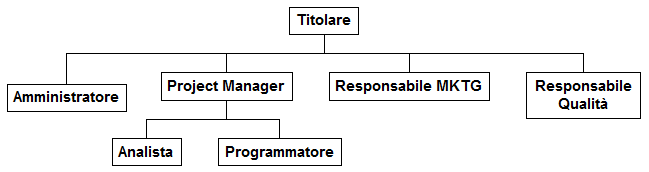
\includegraphics[width=\textwidth]{OBS}
	\caption{Organizational Breakdown Structure}
\end{figure}


Come si evince dal diagramma, tutti i responsabili sono a capo del titolare dell'azienda. Essendo infatti una piccola azienda il controllo, pur essendo distribuito rimane comunque sotto la supervisione del titolare.
Il Project Manager è invece a capo dell' Analista e del Programmatore. 
 
Si noti che tutte le risorse umane di cui dispone l'azienda sono impiegate nel progetto.

	\subsubsection{Titolare}
	Il Titolare è colui che possiede l'azienda (in tutto o in parte).
	\subsubsection{Amministratore}		
	L'amministratore è una figura molto importante dal punto di vista organizzativo. Ogni decisione deve essere approvata da 	tale figura e perciò deve essere messo al corrente di cosa succede sia nelle attività ordinarie che in quelle di progetto.
	Egli è responsabile dell'efficienza e dell'operatività dell'ambiente di sviluppo. Controlla inoltre versioni e configurazioni del prodotto.
	\subsubsection{Project Manager}
	Il Project Manager ricopre un ruolo determinante nella gestione dei progetti. Esso infatti è responsabile della valutazione, pianificazione, realizzazione e controllo di un progetto.
	I suoi compiti più importanti sono:
	\begin{itemize}
		\item Valutazione di costi e benefici del progetto
		\item Pianificazione del progetto
		\item Pianificazione e gestione dei rischi di progetto
		\item Valutazione dello stato di avanzamento del progetto

	\end{itemize}

\subsubsection{Responsabile Marketing}
	Questa figura si occupa della definizione ed applicazione delle strategie di \inglese{marketing}. Il Responsabile Marketing si interessa delle relazioni con i clienti ed alla promozione delle attività dell'azienda stessa. Tale figura si occupa inoltre, del monitoraggio dei dati di mercato, degli indicatori e dei canali di vendita, al fine di permettere l'identificazione di nuove opportunità di \inglese{business}. La persona che ricopre il ruolo di Responsabile Marketing deve avere ottime capacità relazionali, manageriali e di \inglese{leadership}. 
\subsubsection{Responsabile Qualità}	
	La qualità è fondamentale per avere successo nei progetti. Oggi è una proprietà irrinunciabile, sia per clienti che fornitori. Per i clienti si tratta infatti di un'assicurazione sul prodotto/servizio che acquistano e per i fornitori, invece, costituisce  un punto di distinzione rispetto ai concorrenti.
Pur essendo una piccola azienda, si punta al raggiungimento della qualità, tramite l'adeguamento allo standard ISO/IEC 9001.
Nell'ambito dei progetti aziendali il Responsabile Qualità deve assicurare l'attuazione dei processi volti a garantire il rilascio di un prodotto/servizio che rispetta tutti i requisiti di qualità stabiliti.
	 
\subsubsection{Analista}
	L'Analista ha un ruolo fondamentale nella fase iniziale del progetto. Tale figura deve infatti effettuare lo studio di fattibilità preoccupandosi dell'aspetto tecnico. Nel caso di specie l'Analista ricopre un ruolo molto importante anche nella fase di sviluppo. Egli sarà infatti, una delle persone addette alla valutazione dei \inglese{software} esistenti nel mercato e perciò  dalla sua stima dipende in gran parte il successo o il fallimento del progetto.

\subsubsection{Programmatore}
	 Tale ruolo, in generale, dovrebbe semplicemente seguire le direttive di un Progettista per generare il codice finale del prodotto. In questo progetto, essendo l'azienda molto piccola, egli avrà il compito di supportare l'Analista nello studio di fattibilità e di analizzare i \inglese{software} avvalendosi della sua personale esperienza.




\subsection{Matrice delle Responsabilità}
La rappresentazione delle assegnazioni delle responsabilità tramite una matrice permette la definizione del flusso di comunicazioni all'interno della struttura organizzativa del progetto. La matrice, permette infatti, di individuare all'interno dell'organizzazione non solo i responsabili di una certa attività ma anche quei soggetti che devono essere consultati o informati.

\clearpage

\begin{figure}[!h]
  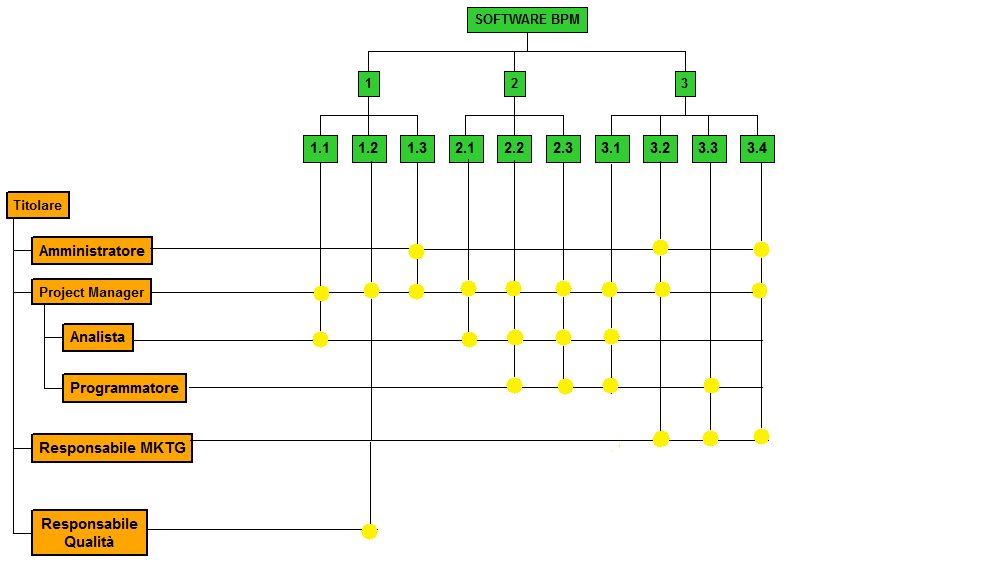
\includegraphics[width=1.6\textwidth]{WBS_OBS}
	\caption{Matrice delle Responsabilità e WBS}
	\label{fig: WBS_OBS}
\end{figure} 

\clearpage
\begin{figure}[!h]
  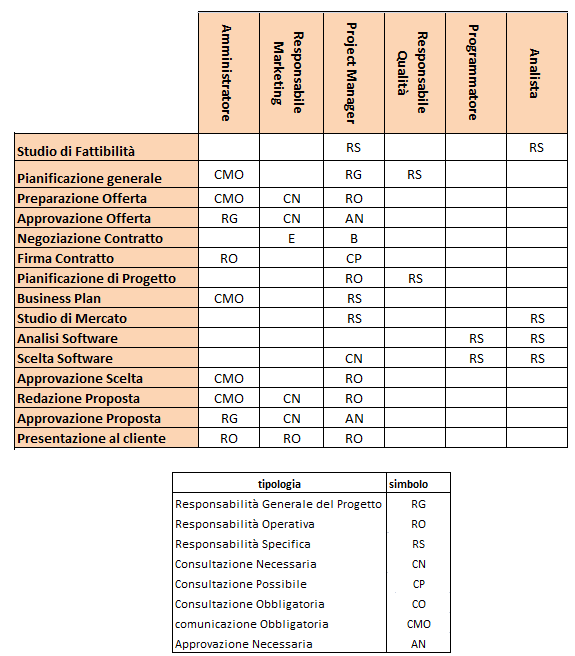
\includegraphics[width=1.5\textwidth]{matrice}
  	\label{fig: MATR}
	\caption{Matrice delle Responsabilità}
\end{figure}

La figura \ref{fig: WBS_OBS} illustra come la matrice delle responsabilità rappresenta l'incrocio tra la WBS e l'OBS. Il diagramma chiarisce infatti chi fa cosa.
La figura \ref{fig: MATR} rappresenta invece la matrice delle responsabilità in modo da individuare anche la specifica responsabilità di ogni figura. Si noti che tale matrice contiene attività molto specifiche, come l'Approvazione, che non si è ritenuto importante inserire nel WBS. Inoltre si fa notare che per attività di Pianificazione Generale si intende una pianificazione poco precisa che ha il solo fine di capire se l'azienda poteva candidarsi per il capitolato. Infine, per quanto riguarda l'attività di Preparazione Offerta si intende la candidatura stessa del \inglese{team} mentre la Firma del Contratto si riferisce all'approvazione da parte del docente.



\subsection{Resource Breakdown Structure}
Una volta definite quali sono le attività da svolgere e chi ne è responsabile è buona norma effettuare la pianificazione di tutte le risorse necessarie alla svolgimento del progetto, sia umane che strumentali.
Tale organizzazione viene effettuata con lo strumento di pianificazione Resource Breakdown Structure (RBS).
Lo scopo principale di RBS è esplicitare tutte le risorse necessarie e le relazioni che intercorrono tra esse, organizzando queste informazioni in un diagramma gerarchico ad albero e classificandole per categoria.


\begin{figure}[!h]
  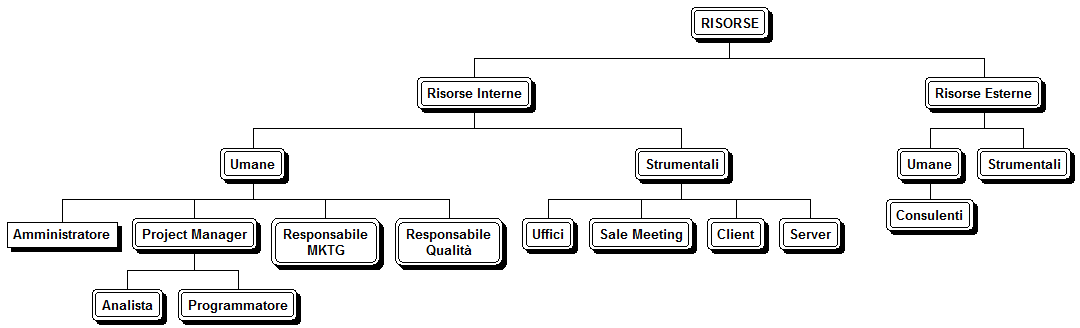
\includegraphics[width=1.5\textwidth]{RBS}
  	\label{fig:RBS}
	\caption{Resource Brakedown Structure}
\end{figure}




Come si evince dal diagramma, le risorse necessarie sono state suddivise gerarchicamente in interne ed esterne, e a loro volta in umane e strumentali. Tale suddivisione permettere di capire dove collocare ogni risorsa necessaria al progetto.

Si noti che vengono considerate esclusivamente le risorse che comportano un costo di cui si dovrà rientrare con gli utili generati dal progetto. Di conseguenza non sono menzionate risorse come \inglese{software} con licenza gratuita.





\subsection{Pianificazione Temporale}
Per la pianificazione temporale si utilizza il diagramma di Gantt.
Tale diagramma rappresenta infatti l'evoluzione del progetto su scala temporale. Il Gantt costituisce non solo un ottimo strumento di pianificazione ma anche un buon strumento di controllo che permette in ogni momento di verificare lo stato di avanzamento del progetto rispetto a tempi ed attività pianificate.


Esso è costituito da un asse orizzontale, sul quel viene rappresentato l'arco temporale totale del progetto e un asse verticale, sul quale sono rappresentate tutte le attività ed i singolo WP che costituiscono il progetto.

\clearpage

\begin{figure}[!h]
  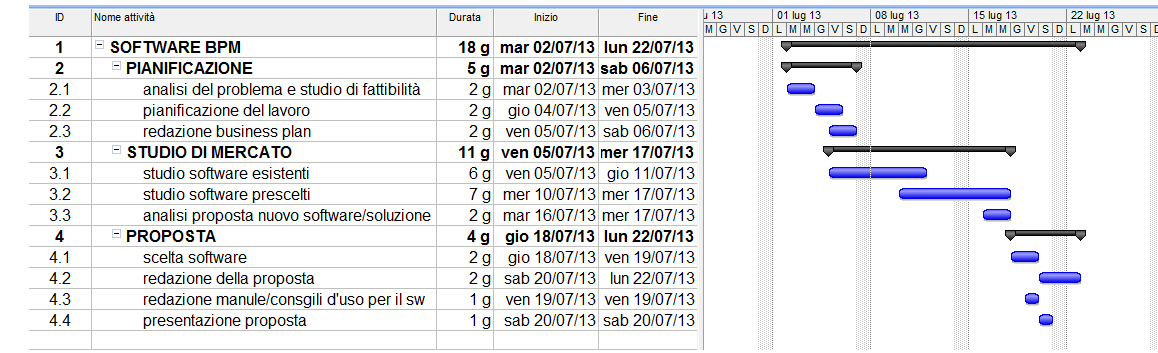
\includegraphics[width=\textwidth]{gantt}	
  	\label{fig:gantt}
	\caption{Diagramma di Gantt}
\end{figure}



\section{Aspetto Economico Finanziario}
Il lato economico costituisce l'aspetto primario di ogni organizzazione che abbia scopo di lucro.
È infatti fondamentale avere un utile sufficientemente remunerativo alla fine del progetto. A tale scopo è finalizzata la stima dei costi relativi al progetto. Tale attività è molto delicata in quanto da essa dipende il reale utile che si ottiene. Infatti, se vi è una sottostima dei costi, l'azienda non avrà utile e nel caso peggiore avrà una perdita. È anche vero, però, che se vi è una sovrastima dei costi, l'azienda non potrà essere competitiva nel mercato.
Il processo di stima avviene calcolando il costo per ogni WP individuato durante il processo di creazione del WBS.
\subsection{Ruoli e Costo }
La seguente tabella espone i costi orari per ogni ruolo individuato.
\begin{figure}[!htb]
\centering
  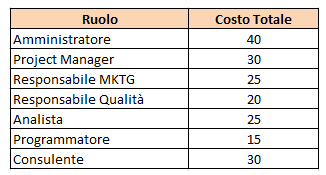
\includegraphics[width=0.55\textwidth]{ruoli}	
  	\label{fig:ruoli}
	\caption{Tabella dei Costi e Ruoli}
\end{figure}

Si noti che tutte le risorse sono interne ad eccezione del consulente. 











\subsection{Costi per Attività}

	

\subsubsection{Pianificazione}
Per l'attività di Pianificazione il costo è previsto è di \textbf{ \text{\euro}1.470,00 }\\	
I costi per ogni WP della Pianificazione sono riassunti nella seguente tabella.
\begin{table}[!h]
\centering
\begin{tabular}{|l|c|c|c|c|c|c|c|}
\hline
\textbf{Attività}& \textbf{AM} & \textbf{RMKTG} & \textbf{PM} & \textbf{RQ} & \textbf{PRG} & \textbf{AN} & \textbf{Costo}  \\ 
              
\hline
analisi del problema e studio di fattibilità  & & & 5& & & 8& \text{\euro} 350,00\\
pianificazione del lavoro	 				  & & &	16&	6& & & \text{\euro} 600,00 \\	
redazione Businee Plan						& 1 & &16& & & &  	\text{\euro} 520,00 \\			  
\hline
PIANIFICAZIONE   							& 1 & &37 &	6 &	&	8 &	\textcolor{red}{ \text{\euro}1.470,00 }\\		 
\hline
\end{tabular}
\caption{costo Pianificazione}\label{tab:pianificazione}
\end{table}
 


\subsubsection{Studio di Mercato}

Per l'attività di Studio di Mercato il costo è previsto è di \textbf{ \text{\euro}2.300,00 }\\	
I costi per ogni WP della Studio di Mercato sono riassunti nella seguente tabella.


\begin{table}[!h]
\centering
\begin{tabular}{|l|c|c|c|c|c|c|c|}
\hline
\textbf{Attività}& \textbf{AM} & \textbf{RMKTG} & \textbf{PM} & \textbf{RQ} & \textbf{PRG} & \textbf{AN} & \textbf{Costo}  \\ 
              
\hline
studio software esistenti & & & 1& & 24& 23& \text{\euro} 965,00\\
studio software prescelti	 				  & & &	&	&40 &16 & \text{\euro} 1.000,00 \\	
 \parbox{162 px}{analisi proposta nuovo software / soluzione ibrida} 					  & & &2 & 	&5	&  8  &  	\text{\euro} 335,00 \\			  
\hline
STUDIO DI MERCATO  							& 1 &  &3 & &69	&47	&	\textcolor{red}{ \text{\euro}2.300,00 }\\		 
\hline
\end{tabular}
\caption{costo Studio di Mercato}\label{tab:mercato}
\end{table}







\subsubsection{Proposta}
Per l'attività di Redazione della Proposta il costo è previsto è di \textbf	{ \text{\euro} 905,00 }	
I costi per ogni WP della Redazione della Proposta sono riassunti nella seguente tabella.


\begin{table}[!h]
\centering
\begin{tabular}{|l|c|c|c|c|c|c|c|}
\hline
\textbf{Attività}& \textbf{AM} & \textbf{RMKTG} & \textbf{PM} & \textbf{RQ} & \textbf{PRG} & \textbf{AN} & \textbf{Costo}  \\ 
              
\hline

scelta software			& & & 3&	& 7&	6& 	\text{\euro} 345,00 \\
redazione della proposta & 1&	8&	6& & & & 	 \text{\euro} 420,00 \\
redazione manuale / consgili d'uso & & & & & 					4 && 	\text{\euro} 60,00 \\	
presentazione proposta		 & & 2&  	1	& & 	& & 		 \text{\euro} 80,00 \\	

	  
\hline
PROPOSTA  							& 1  &10 &10& &	4&	6&	\textcolor{red}{ \text{\euro} 905,00 }\\		 
\hline
\end{tabular}
\caption{costo Redazione Proposta}\label{tab:proposta}
\end{table}	
	
	
\subsubsection{Consulenza}
	
	
Si noti che nelle tabelle relative alle attività non sono inclusi i costi relativi alla figura del consulente. Il \inglese{team} ha infatti deciso di trattarli a parte. La seguente tabella indica i costi che il \inglese{team}prevede di sostenere per le spese di consulenza in ogni fase.
	
\clearpage
\begin{table}[!h]
\centering
\begin{tabular}{|l|c|c|}
\hline
\textbf{Attività}& \textbf{Consulente} & \textbf{Costo}  \\ 
              
\hline

PIANIFICAZIONE		& 1& \text{\euro} 30,00 \\
STUDIO DI MERCATO 	& 5& \text{\euro} 150,00 \\
PROPOSTA 			& &	\text{\euro} 60,00 \\	
\hline
Totale				& 6& \text{\euro} 180,00 \\	
\hline
\end{tabular}
\caption{costo Consulenza}\label{tab:consulenza}
\end{table}

Come si evince dalla tabella il costo stimato per le spese di consulenza è di \textbf	{ \text{\euro} 180,00 }	

\subsection{Costo Totale}

Il costo totale stimato ammonta quindi a \textbf	{ \text{\euro} 4855,00 }.
Sarà perciò necessario richiedere un corrispettivo maggiorato di una cifra che possa essere sufficientemente remunerativa ma che allo stesso tempo permetta all'azienda di essere competitiva nel mercato.









\section{Gestione dei Rischi}
Un rischio è un evento incerto o una condizione di incertezza che se accade determina un effetto positivo o negativo sull'obbiettivo di progetto.
La gestione dei rischi è fondamentale in un progetto. Infatti, da una gestione corretta o errata del rischio dipende il successo o il fallimento del progetto.
È quindi necessario individuare quali rischi possono verificarsi durante il progetto e pianificare tecniche e strategie per evitare o, nel caso peggiore, mitigare tali rischi.

La valutazione dei rischi non deve essere un processo statico ma dinamico. Non è infatti sufficiente individuare rischi e tattiche all'inizio del progetto ma è necessario effettuare azioni di controllo costanti. 

\subsection{Analisi dei rischi}


Per rendere efficace l'analisi di ogni rischio si è deciso di quantificarlo mediante un apposita scala di valutazione sia dal punto di vista della probabilità che il rischio si manifesti (livello), sia il suo grado di incidenza sul progetto stesso (impatto).

\begin{table}[h!]
\centering
\begin{tabular}{|l|c|}
\hline
Probabilità& Descrizione\\
\hline
ALTA & probabilità elevata che si verifichi\\
MEDIA & probabilità equivalente nel verificarsi o meno\\
BASSA & probabilità bassa che si verifichi\\
\hline
\end{tabular}
\caption{Probabilità e Descrizione probabilità di un rischio}\label{tab:livellorischi}
\end{table}
\begin{table}[h!]
\centering
\begin{tabular}{|c|c|}
\hline
Scala& Descrizione  \\
\hline
5 & conseguenze molto gravi\\
4 & conseguenze gravi\\
3 & conseguenze medio-gravi\\
2 & conseguenze minimali\\
1 & nessuna/lievi conseguenze\\
\hline
\end{tabular}
\caption{Scala e descrizione delle conseguenze di un rischio}\label{tab:impattorischi}
\end{table}


\subsection{Rischi relativi al Personale}

\begin{description}
	\item{\scshape\bfseries Analisi:} durante la realizzazione del progetto è probabile che alcuni membri del team siano soggetti a problemi fisiologici e/o sovvengano impegni personali improrogabili che porterebbero ad una sicura modifica della pianificazione del lavoro collettivo. L'impatto di tale rischio è variabile in base al soggetto mancante, in quanto può essere assegnato ad un'attività più o meno importante all'interno del progetto. 
	\item{\scshape\bfseries Probabilità:} MEDIA
	\item{\scshape\bfseries Impatto:} variabile
	\item{\scshape\bfseries Strategia di Gestione:} per mitigare gli effetti di tali fenomeni è ragionevole prima di tutto pianificare i tempi di lavoro personali in modo da lasciare un lasco temporale tra un attività e l'altra.
Purtroppo, data la scarsità di tempo a disposizione, si dispone in questo caso di poco tempo margine. Tuttavia, essendo il periodo che impegnerà il \inglese{team} breve, vi è una cospicua probabilità che le attività procedano come pianificate.
	
Ovviamente anche adottando tali accorgimenti si potrà generare la situazione in cui un componente risulti impossibilitato a svolgere il proprio compito, in tal caso è buona norma che tutti i membri siano ben preparati (conoscenza del dominio e delle metodologie di lavoro) nel caso sia necessaria la sostituzione momentanea del soggetto.
\end{description}

\subsection{Rischi relativi alla Tecnologia}
\begin{description}
	\item{\scshape\bfseries Analisi:} per ovvie ragioni di inesperienza da parte di tutto il team buona parte delle competenze tecnologiche richieste per la realizzazione del progetto risultano sconosciute.
	\item{\scshape\bfseries Probabilità:} ALTA 
	\item{\scshape\bfseries Impatto:} 3 
	\item{\scshape\bfseries Strategia di Gestione:} le lacune saranno colmate tramite la personale consultazione di materiale presente in rete. Inoltre, ogni persona provvederà ad aggiornare costantemente gli altri membri del \inglese{team} sul lavoro svolto.
	
	
	
\subsection{Rischi relativi all'Errata Stima di Risorse}
\begin{description}
	\item{\scshape\bfseries Analisi:} l'errata pianificazione del lavoro fa parte dell'ovvia inesperienza del team, e in particolare di chi ricopre il ruolo di Project Manager. Tali errori possono portare ad uno sbilanciamento dei costi (sia in eccesso che in difetto) che andrà ad incidere sul bilancio finale.
	\item{\scshape\bfseries Probabilità:} MEDIA
	\item{\scshape\bfseries Impatto:} 3 
	\item{\scshape\bfseries Strategia di Gestione:} per mitigare gli effetti di tali rischi il \inglese{team} ha cercato di fare ricerche molto approfondite sugli argomenti e ha effettuato una pianificazione leggermente ``pessimistica''. In questo modo viene ridotto la probabilità di incorrere ad eventuali perdite che inclinerebbero lo stato economico-finanziario dell'azienda.
\end{description}	
	
	
\subsection{Rischi relativi al Mercato}
\begin{description}
	\item{\scshape\bfseries Analisi:} il \inglese{team} non ha nessuna esperienza sulla situazione di mercato dei \inglese{software} BPM. Tale carenza, purtroppo, può incidere molto sulla tempistica di realizzazione del progetto.
	\item{\scshape\bfseries Probabilità:} ALTA
	\item{\scshape\bfseries Impatto:} 3 
	\item{\scshape\bfseries Strategia di Gestione:} per mitigare gli effetti di tali rischi il \inglese{team} potrà avvalersi di eventuali consulenti e dell'aiuto del docente.
\end{description}	
	
	

\end{description}
\end{document}

